\documentclass[a4paper,12pt]{article} % тип документа

%  Русский язык
\usepackage[T2A]{fontenc}			% кодировка
\usepackage[utf8]{inputenc}			% кодировка исходного текста
\usepackage[english,russian]{babel}	% локализация и переносы

\usepackage{graphicx}               % импорт изображений
\usepackage{wrapfig}                % обтекаемые изображения
\graphicspath{{pictures/}}          % обращение к подкаталогу с изображениями
\usepackage[14pt]{extsizes}         % для того чтобы задать нестандартный 14-ый размер шрифта
\usepackage[warn]{mathtext}         % русский язык в формулах
\usepackage{indentfirst}            % indent first
\usepackage[margin = 25mm]{geometry}% отступы полей
\usepackage[table,xcdraw]{xcolor}   % таблицы
\usepackage{amsmath,amsfonts,amssymb,amsthm,mathtools} % Математика
\usepackage{wasysym}                % ???
\usepackage{upgreek}                % ???  
\usepackage{caption}
\captionsetup{labelsep=period}
\usepackage{gensymb} % degree symbol
\usepackage[unicode, pdftex]{hyperref}
\definecolor{urlcolor}{HTML}{0000FF}
\hypersetup{pdfstartview=FitH,urlcolor=urlcolor, colorlinks=true}



\begin{document}
\section*{Обработка экспериментальных данных}
\setcounter{page}{26}

\begin{enumerate}
	\item Загрузим данные из \href{file:Data.xlsx}{файла.}
	
	\item Зная объём «запертого» в сильфоне воздуха $V_{\text{с}} = 265$ мл, определим,
	пользуясь законом Бойля-Мариотта, полный объём установки, высоковакуумной части (камера К), форвакуумной магистрали и самого насоса ТМН.
	
	$p_{0}V_{\text{c}} + p_{\text{пред}}V_{\text{K}} = p_{1}(V_{\text{c}} + V_{\text{K}})$,
	
	
	$V_{\text{K}} = V_{\text{c}}\cdot\frac{p_{0} - p_{1}}{p_{1} - p_{\text{пред}}}$ = 955 мл,
	
	где $p_{0}$ = 10$^3$ мбар - это атмосферное давление, $p_{1}$ = 2,2$\cdot 10^2$ мбар, $p_{\text{пред}}$ = 3,5 мбар.
	
	Относительные ошибки значений давлений (по паспортам приборов): $\delta_{p_{1}} = $ 0,05; $\delta_{p_{\text{пред}}} = $ 0,15.
	
	$\sigma_{V_{\text{K}}} = V_{\text{K}}\sqrt{\delta_{p_{1}}^2 + \delta_{p_{\text{пред}}}^2} = $151 мл.
	
	\begin{center}
	\framebox{$V_{\text{K}} = (955 \pm 151)\text{ мл}$}
	\end{center}

	Аналогично:
	
	$p_{1}(V_{\text{c}} + V_{\text{K}}) + p_{\text{пред}}V_{\text{маг+нас}} = p_{2}(V_{\text{c}} + V_{\text{K}} + V_{\text{маг+нас}})$,
	
	где $p_{2} =$ 1,7 $\cdot 10^2$ мбар.
	
	Получаем:
	
	$V_{\text{маг+нас}} = (V_{\text{c}} + V_{\text{K}})\cdot\frac{p_{1} - p_{2}}{p_{2} - p_{\text{пред}}} = 366$ мл.
	
	Относительные ошибки: $\delta_{p_{1}} = \delta_{p_{2}} = $ 0,05; $\delta_{p_{\text{пред}}} = $ 0,15. 
	
	$\sigma_{\text{маг+нас}} = V_{\text{маг+нас}}\sqrt{\delta_{p_{1}}^2 + \delta_{p_{2}}^2 + \delta_{p_{\text{пред}}}^2 + \left(\frac{\sigma_{V_{\text{K}}}}{V_{\text{K}}}\right)^2} = $ 84 мл.
	
	\begin{center}
	\framebox{$V_{\text{маг+нас}} = (366 \pm 84)\text{ мл} $}
	\end{center}
	
	Тогда общий объем установки: $V_{\text{уст}} = V_{\text{c}} + V_{\text{K}} + V_{\text{маг+нас}} = (265 + 955 + 366)$ мл = 1586 мл.
	
	$\sigma_{V_{\text{уст}}} = V_{\text{уст}}\sqrt{\left(\frac{\sigma_{V_{\text{K}}}}{V_{\text{K}}}\right)^2 + \left(\frac{\sigma_{V_{\text{маг+нас}}}}{V_{\text{маг+нас}}}\right)^2} = $ 342 мл.
	
	\begin{center}
	\framebox{$V_{\text{уст}} = (1586 \pm 342) \text{ мл}$}
	\end{center}
	
	\item Оценим эффективную скорость откачки системы форвакуумным насосом в области, где она почти постоянна: из файла возьмем данные зависимости давления в камере К от времени откачки насосом ДН. По зависимости $\ln{P}(t)$ (график 1) определим постоянную времени откачки $\tau$ в диапазоне давлений $10-100$ мбар.
	
	$P(t) = P_{0}e^{-\frac{t}{\tau}}$;
	
	$\ln{P} = \ln{P_{0}} - \frac{t}{\tau}$;
	
	Используя МНК, получаем следующие значения:
	
	$k = -\frac{1}{\tau} = -$0,058 c$^{-1}$;
	
	$\sigma_{k} = $ 0,002 c$^{-1}$.
	
	\vspace{5mm}
	$\tau = -\frac{1}{k} = $ 17,2 c;
	
	$\sigma_{\tau} = \tau \cdot \frac{\sigma_{k}}{|k|} = $ 0,6 c;

	\begin{center}
	\framebox{$\tau = (17,2 \pm 0,6)\text{ c}$}
	\end{center}

	\begin{figure}[h!]
		\centering
		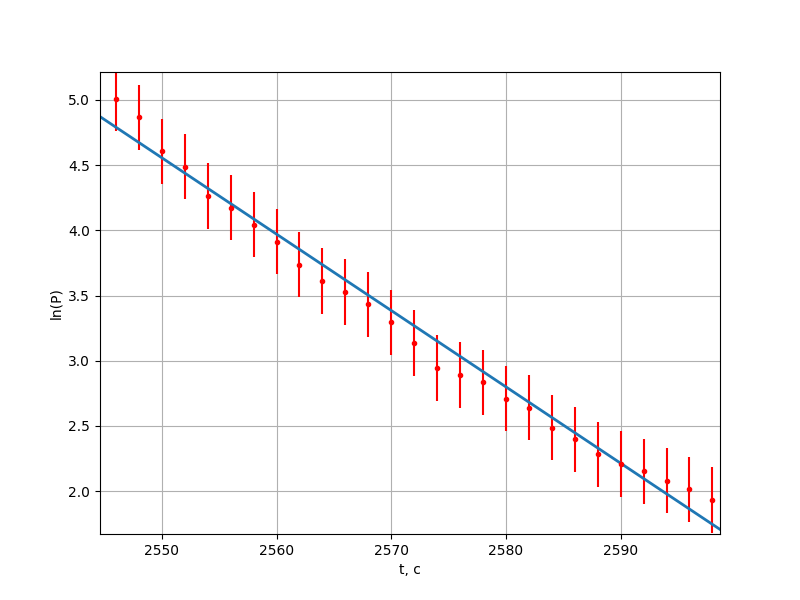
\includegraphics[scale=0.7]{Pictures/lnP(t) ДН.png}
		\caption*{График 1. По оси абсцисс - время в секундах от начала работы.}
	\end{figure}
	

\newpage
Зная объём камеры К установки $V_{\text{K}} = 955$ мл, рассчитаем эффективную скорость её откачки $S_{0}$:


$S_{0} = \frac{V_{\text{K}}}{\tau} = \frac{955}{17,2} \text{ }\frac{\text{мл}}{\text{с}} = 55 \text{ }\frac{\text{мл}}{\text{с}}$.

$\sigma_{S_{0}} = S_{0}\sqrt{\left(\frac{\sigma_{V_{\text{K}}}}{V_{\text{K}}}\right)^2 + \left(\frac{\sigma_{\tau}}{\tau}\right)^2} = 9\text{ }\frac{\text{мл}}{\text{с}}$. 

\begin{center}
	\framebox{$S_{0} = (55 \pm 9)\text{ }\frac{\text{мл}}{\text{с}}$}
\end{center}


Определим суммарную пропускную способность $U$:


$\frac{1}{S_{0}} = \frac{1}{S_{\text{н}}} + \frac{1}{U}$,

где $S_{\text{н}} = 139\text{ }\frac{\text{мл}}{\text{с}}$ - скорость откачки по паспортным данным насоса.

Отсюда получаем:

$U = \frac{S_{\text{н}}S_{0}}{S_{\text{н}} - S_{0}} = 92\text{ }\frac{\text{мл}}{\text{с}}$;

$\sigma_{U} = U \cdot\frac{\sigma_{S_{0}}}{S_{0}} = 15\text{ }\frac{\text{мл}}{\text{с}}$;

\begin{center}
	\framebox{$U = (92 \pm 15)\text{ }\frac{\text{мл}}{\text{с}}$}
\end{center}


\item Оценим эффективную скорость откачки системы турбомолекулярным насосом в области, где она почти постоянна: из файла возьмем данные зависимости давления в камере К от времени откачки насосом ТМН. По зависимости $\ln{P}(t)$ (график 2) определим постоянную времени откачки $\tau$ в диапазоне давлений $10^{-5}-10^{-3}$ мбар.

	$P(t) = P_{0}e^{-\frac{t}{\tau}}$;

	$\ln{P} = \ln{P_{0}} - \frac{t}{\tau}$;

	Пользуясь МНК, получаем следующие значения:

	$k = -\frac{1}{\tau} = -$0,027 c$^{-1}$;

	$\sigma_{k} = $ 0,002 c$^{-1}$.

	\vspace{5mm}
	$\tau = -\frac{1}{k} = $ 37,0 c;

	$\sigma_{\tau} = \tau \cdot \frac{\sigma_{k}}{|k|} = $ 2,8 c;

	\begin{center}
		\framebox{$\tau = (37,0 \pm 2,8)\text{ c}$}
	\end{center}

\newpage
\begin{figure}[h!]
	\centering
	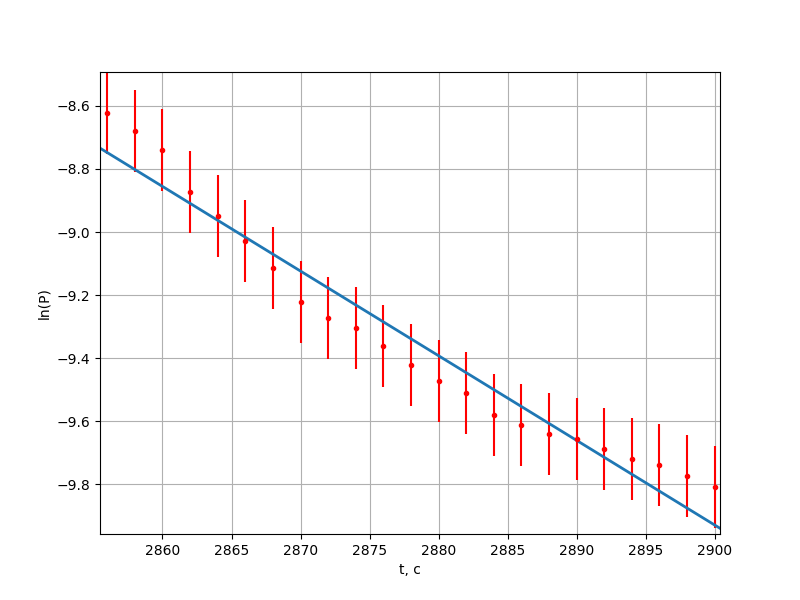
\includegraphics[scale=0.8]{Pictures/lnP(t) ТМН.png}
	\caption*{График 2. По оси абсцисс - время в секундах от начала работы.}
\end{figure}


Зная объём камеры К установки $V_{\text{K}} = 955$ мл, рассчитаем эффективную скорость её откачки $S_{0}$:

$S_{0} = \frac{V_{\text{K}}}{\tau} = \frac{955}{37}\text{ }\frac{\text{мл}}{\text{с}} = 26\text{ }\frac{\text{мл}}{\text{с}}$;

$\sigma_{S_{0}} = S_{0}\sqrt{\left(\frac{\sigma_{V_{\text{K}}}}{V_{\text{K}}}\right)^2 + \left(\frac{\sigma_{\tau}}{\tau}\right)^2} = 2\text{ }\frac{\text{мл}}{\text{с}}$.

\begin{center}
	\framebox{$S_{0} = (26 \pm 2)\text{ }\frac{\text{мл}}{\text{с}}$}
\end{center}


Определим суммарную пропускную способность $U$:


$\frac{1}{S_{0}} = \frac{1}{S_{\text{н}}} + \frac{1}{U}$,

где $S_{\text{н}} = 67000\text{ }\frac{\text{мл}}{\text{с}}$ - скорость откачки по паспортным данным насоса.

Отсюда получаем:

$U = \frac{S_{\text{н}}S_{0}}{S_{\text{н}} - S_{0}} \approx 26\text{ }\frac{\text{мл}}{\text{с}}$;

$\sigma_{U} = U \cdot\frac{\sigma_{S_{0}}}{S_{0}} = 2\text{ }\frac{\text{мл}}{\text{с}}$;

\begin{center}
	\framebox{$U = (26 \pm 2)\text{ }\frac{\text{мл}}{\text{с}}$}
\end{center}


Сравним экспериментальные данные с расчетными значениями:

$U_{\text{отв}} = \frac{1}{4}\pi R_{\text{отв}}^2 \sqrt{\frac{8RT}{\pi \mu}}$,

где $R_{\text{отв}}$ - радиус отверстия. В нашем случае $R_{\text{отв}} \thicksim 1$ см.

Тогда:

$U_{\text{отв}} = \frac{1}{4}\cdot 3,14 \cdot 0,01^2 \sqrt{\frac{8\cdot 8,314\cdot 293}{3,14\cdot 0,029}} = 36,3 \text{ }\frac{\text{мл}}{\text{c}}$.


Как видим, рассчитанные и полученные значения достаточно близки.



\item Определим уровень течей по ухудшению вакуума после перекрытия откачки насосом ТМН. Из файла возьмем данные зависимости давления в камере К от времени натекания после перекрытия откачки шибером ШЗ.


Рассчитаем натекание $Q_{\text{н}}:$


$Q_{\text{н}} = V_{\text{K}}\frac{P_{\text{кон}} - P_{\text{нач}}}{\Delta t} = 955\cdot\frac{3\cdot 10^{-3} - 3,9\cdot 10^{-5}}{472}\text{ }\frac{\text{мл}\cdot\text{мбар}}{\text{c}} \approx 0,006\text{ }\frac{\text{мл}\cdot\text{мбар}}{\text{c}}$.


$Q = P_{1}S_{0} \thicksim 10 \cdot 55 \text{ }\frac{\text{мл}\cdot\text{мбар}}{\text{c}} = 550 \text{ }\frac{\text{мл}\cdot\text{мбар}}{\text{c}}$.

Как мы видим, для заданного выше диапазона давлений условие $Q_{\text{н}}\ll Q$ выполняется.

\newpage
\item Исследуем зависимость мощности турбины ТМН от давления в камере К при создании искусственной течи. Из файла возьмите данные зависимости мощности турбины ТМН от давления в камере К.
Построим графики $W(P)$ при увеличении течей (график 3) и их уменьшении (график 4).

a) Используем МНК и получаем:

Коэффициент наклона $k = 5506\text{ }\frac{\text{Вт}}{\text{мбар}}$

\begin{figure}[h!]
	\centering
	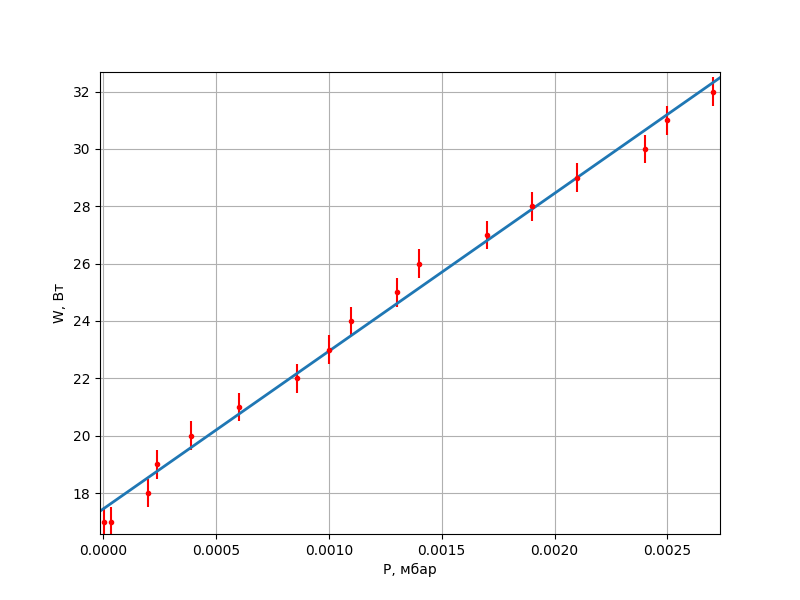
\includegraphics[scale=0.8]{Pictures/W(P) повыш.png}
	\caption*{График 3}
\end{figure}

\newpage
б) Аналогично:

Коэффициент наклона $k = 6225\text{ }\frac{\text{Вт}}{\text{мбар}}$

\begin{figure}[h!]
	\centering
	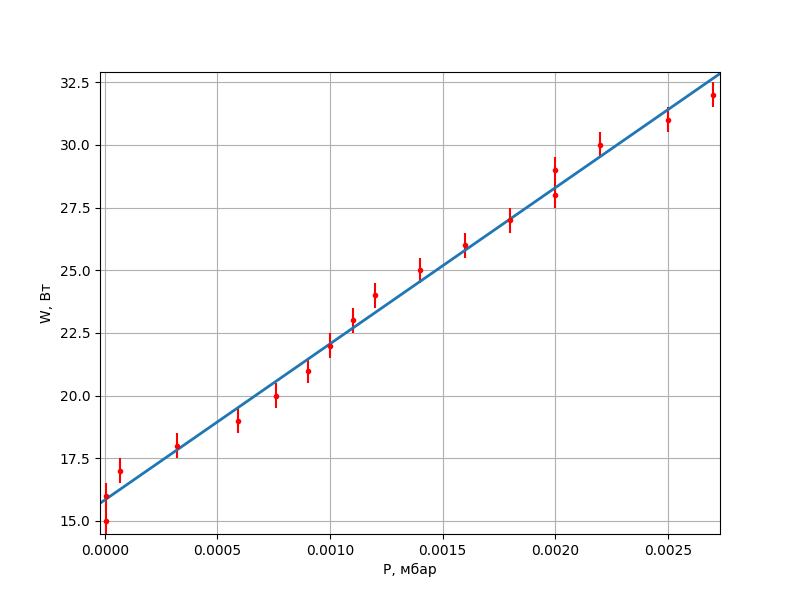
\includegraphics[scale=0.8]{Pictures/W(P) пониж.png}
	\caption*{График 4}
\end{figure}

\item Оценим число Кнудсена для предельных давлений при форвакуумной и высоковакуумной откачке.

Kn = $\frac{\lambda}{d} \thicksim \frac{kT}{\sqrt{2}\pi r^2 P \sqrt[3]{V_{\text{K}}}}$,

где $r \approx 3\cdot 10^{-10}$ м - размер молекулы воздуха.

Для форвакуумной откачки получаем Kn$\thicksim$10$^{-3}$ - гидродинамический режим течения.

Для высоковакуумной откачки - Kn$\thicksim$10$^3$ - кнудсеновский режим течения.

\end{enumerate}

\newpage
\section*{Вывод}
В работе были рассмотрены способы получения и измерения вакуума. В ней были найдены объемы высоковакуумной части установки - $V_{\text{K}} = (955 \pm 151)$ мл, форвакуумной магистрали и ТМН - $V_{\text{маг+нас}} = (366 \pm 84)$ мл. Также были рассчитаны эффективные скорости откачки и пропускные способности: ДН  - $S_{0} = (55 \pm 9) \text{ }\frac{\text{мл}}{\text{c}}$, $U = (92 \pm 15)\text{ }\frac{\text{мл}}{\text{c}}$; ТМН -  $S_{0} = (26 \pm 2)\text{ }\frac{\text{мл}}{\text{c}}$, $U = (26 \pm 2)\text{ }\frac{\text{мл}}{\text{c}}$. Ошибки связаны с неточностью измерений и несовершенством техники измерений.

\end{document}